\documentclass[a4paper]{article}
\usepackage{fontspec}
\usepackage[russian]{babel}
\usepackage{listings}
\usepackage[a4paper]{geometry}
\usepackage{indentfirst}
\usepackage{graphicx}
\usepackage{caption}
\usepackage{float}

\setmainfont{CMU Serif}
\setsansfont{CMU Sans Serif}

\begin{document}

\title{Лабораторная работа 3 по курсу <<Нелинейная динамика и её приложения>>. \\Отчёт.}
\author{Владислав Соврасов\\ 381503м4}
\date{}
\maketitle

\section{Численное интегрирование уравнений методом Эйлера с постоянным шагом}
Пусть необходимо решить численно уравнение вида \(\dot x(t)=f(x,t)\) с начальным
условием \(x(0)=x_0\). \(x(t)\) и \(f(x,t)\) в рассматриваемом уравнении могут быть,
вообще говоря, вектор-функциями. Метод Эйлера имеет простую вычислительную формулу:
\begin{displaymath}
	x_{n+1}=x_n+hf(x_n, h\cdot n),n=\overline{0,s},
\end{displaymath}
где \(h>0\) --- шаг метода.

Рассмотрим работу метода на примере интегрирования уравнений \(\dot x(t) = \pm x, x(0)=1\).
В случае положительной правой части решением уравенения является функция \(x(t)=e^x\).
Метод Эйлера при решении этого уравнения строит последоввательность, которая растёт
как геометрическая прогрессия со знаменателем \(h+1\), в то время, как
последовательность значений функции-решения в узлах сетки является
геометрической прогрессией со знаменателем \(e^h\). \(e^h - 1 - h = h^2/2 + O(h^3)>0\)
прим малом \(h\), поэтому разность между численным и истинным решениями на сетке
будет расти также как геометрическая прогрессия, т.е. экспоненциально. Этот эффект
виден на рис. \ref{fig:euler_exp_plus}.
В случае решения уравнения \(\dot x(t) = - x, x(0)=1\) верны те же самые рассуждения,
но прогрессия здесь будет убывающей (рис. \ref{fig:euler_exp_minus}).

Из рис. \ref{fig:euler_exp_plus}, \ref{fig:euler_exp_minus} также видно, что метод
Эйлера имеет первый порядок сходимости: при уменьшении шага в 10 раз ошибка интегрирования
на отрезке падает примерно в 10 раз.

Далее рассмотрим интегрирование уравнения второго порядка: \(\ddot x + x=0\) при
начальных условиях \(x(0)=1,\dot x(0)=0\). Это уравнение после введения фазовой скорости
\(y(t)=\dot x(t)\) эквивалентно системе:
\begin{displaymath}
	\left\{
  \begin{array}{lr}
    \dot x = y\\
    \dot y = -x
  \end{array}
\right.
\end{displaymath}

Эту систему можно решать методом Эйлера. В качестве ошибки интегрирования рассматривается
абсолютная разность численного и настоящего решений по координате \(x\). Решением
исходного уравнения при заданных начальных условиях является функция \(x(t)=cos(t)\). Как видно
из рис. \ref{fig:euler_system}, ошибка похожа на периодическую функцию, однако со временем
нарастает. Минимумы этой функции соответствуют нулям решения \(x(t)=cos(t)\). Как и на
предыдущих графиках, здесь также подтверждается первый порядок сходимости метода
Эйлера.

\begin{figure}[H]
	\center
	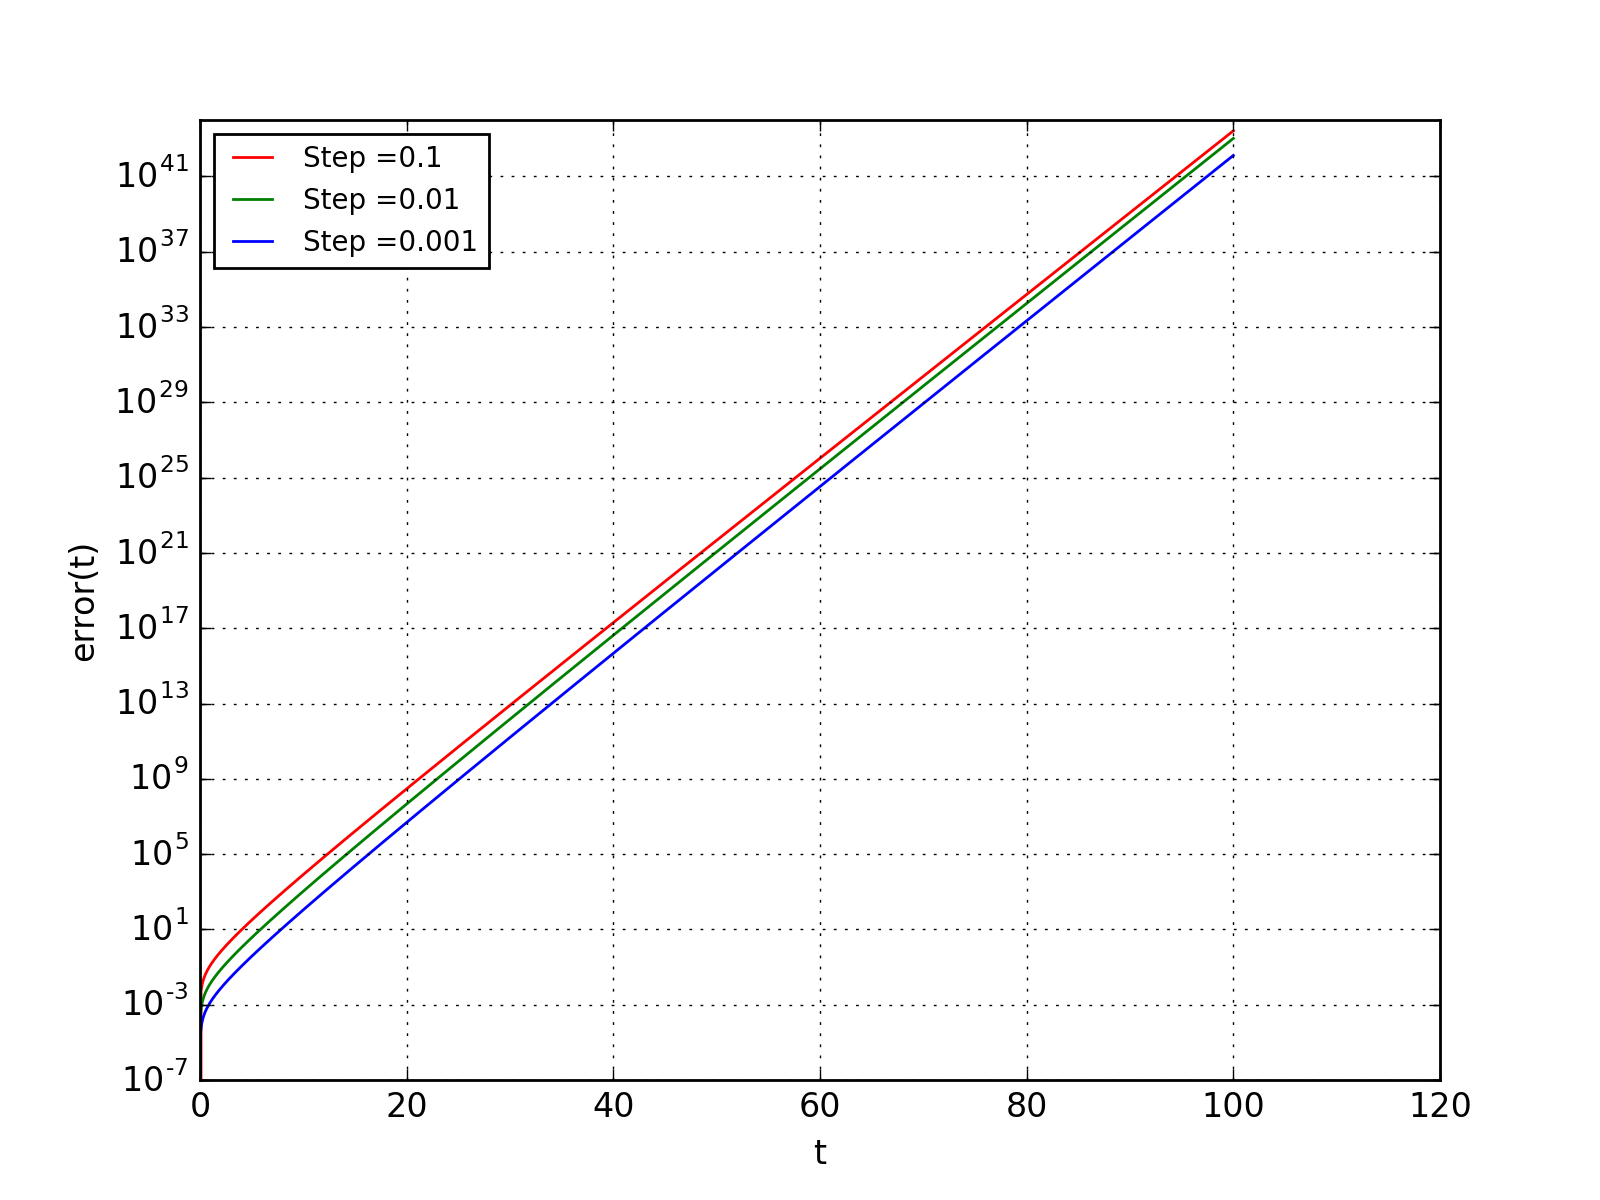
\includegraphics[width=0.75\textwidth]{../pictures/lab3_exp_plus.png}
	\caption{Ошибка интегрирования уравнения \(\dot x(t) = x\) при различных значениях шага}
	\label{fig:euler_exp_plus}
\end{figure}

\begin{figure}[H]
	\center
	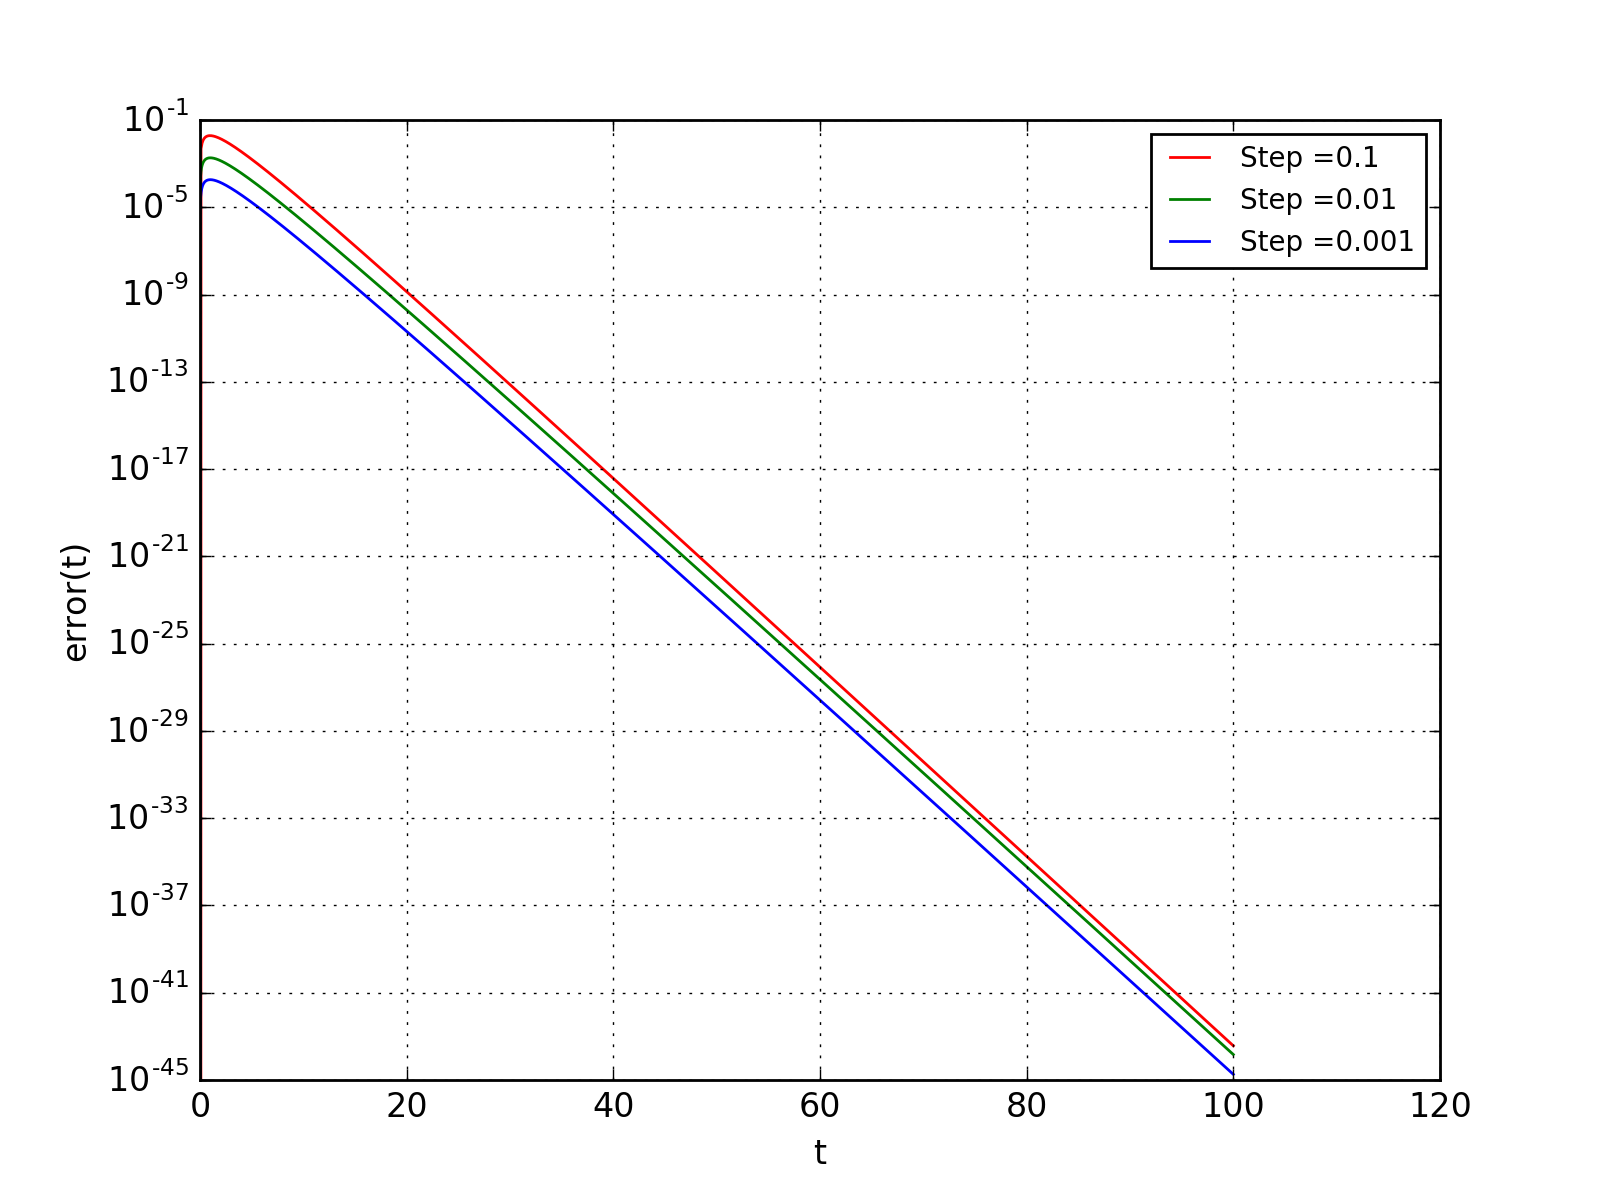
\includegraphics[width=0.75\textwidth]{../pictures/lab3_exp_minus.png}
	\caption{Ошибка интегрирования уравнения \(\dot x(t) = -x\) при различных значениях шага}
	\label{fig:euler_exp_minus}
\end{figure}

\begin{figure}[H]
	\center
  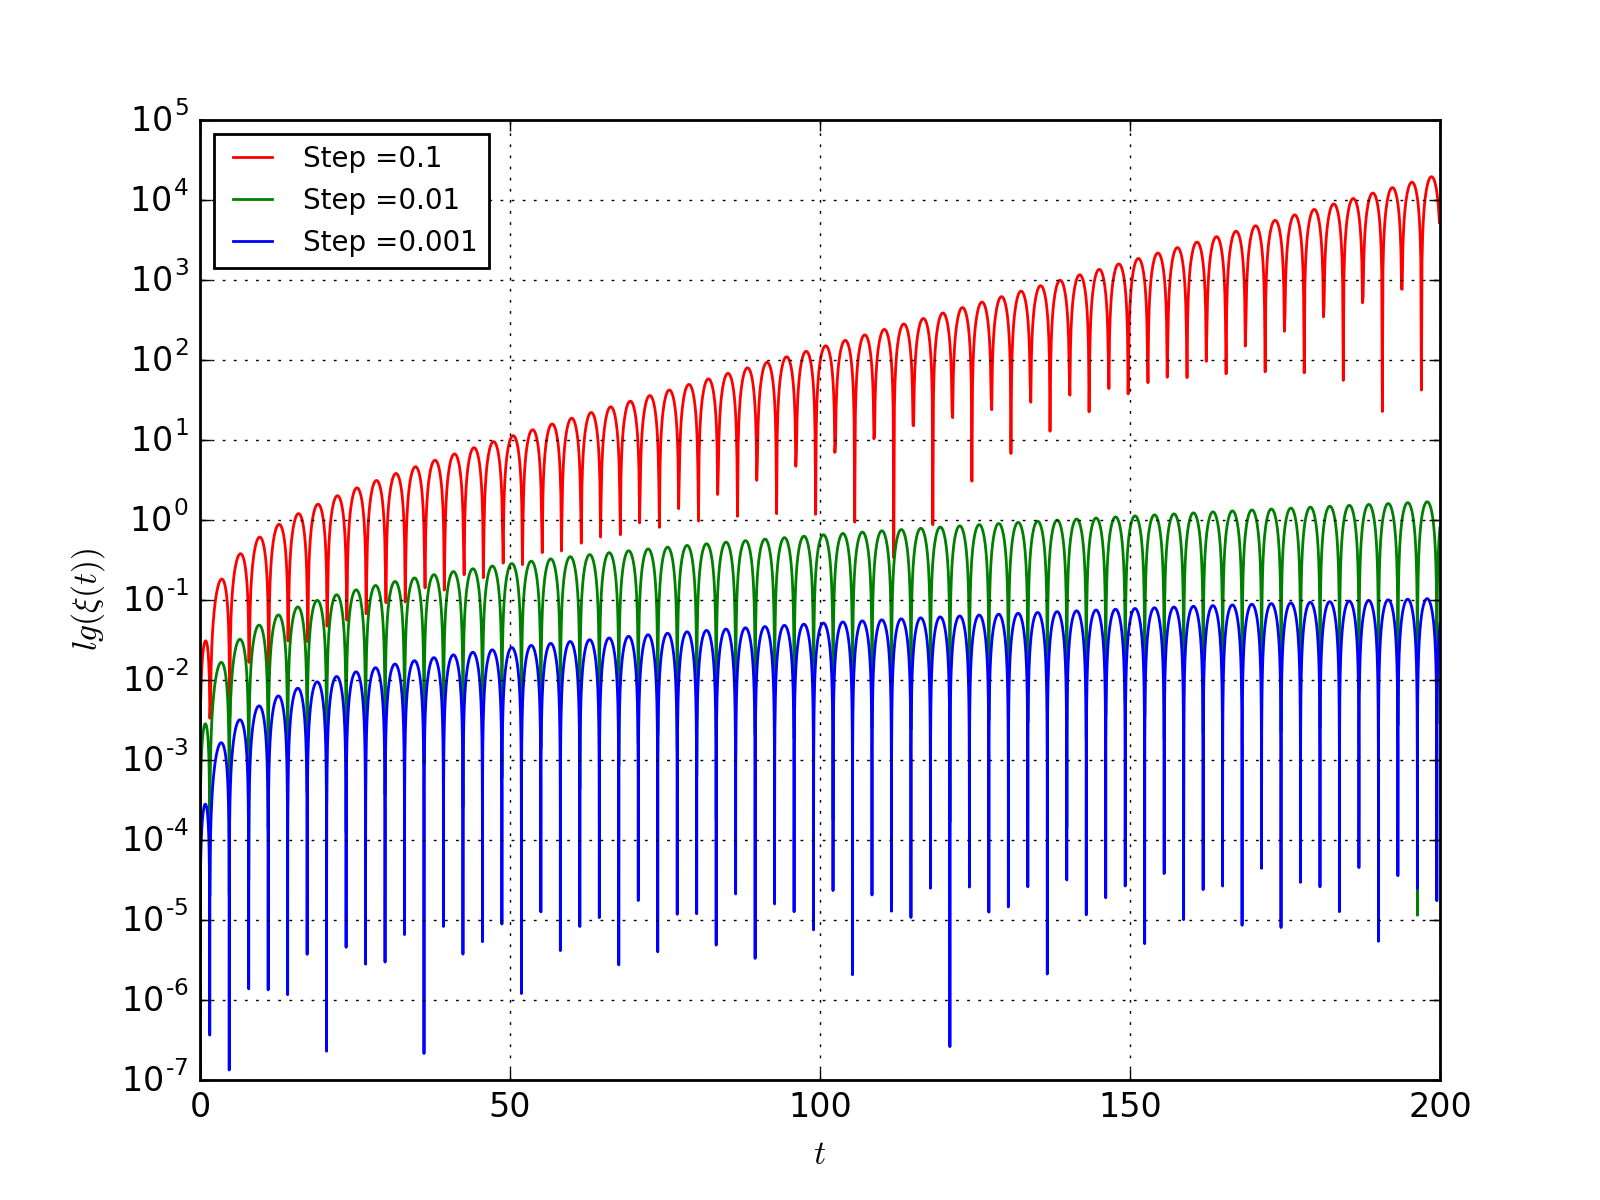
\includegraphics[width=0.75\textwidth]{../pictures/lab3_cons_system.png}
  \caption{Ошибка интегрирования уравнения \(\ddot x(t) +x = 0\) при различных значениях шага}
  \label{fig:euler_system}
\end{figure}

\section{Численное интегрирование системы Рёсслера методом Рунге-Кутты с постоянным шагом}

Рассмотрим систему из трёх уравнений:
\begin{displaymath}
	\left\{
  \begin{array}{lr}
    \dot x = -y - z\\
		\dot y = x + 0.3y \\
    \dot z = 0.3 + (x-5.7)z
  \end{array}
\right.
\end{displaymath}
при начальных условиях \(x(0)=1,y(0)=0,z(0)=100\).

Для численного решения этой системы применялся метод Рунге-Кутты 4го порядка с
постоянным шагом. Точное решение неизвестно, поэтому для оценки ошибки интегрирования
использовалось численное решение, полученное тем же методом, но с вдвое меньшим шагом.
На рис. \ref{fig:rossler_system} показана разность численных решений по норме \(L1\).
Из графика виден четвёртый порядок сходимости метода, а также то, что ошибка интегрирования
изменяется сначала хаотично, а потом становится похожей на периодическую функцию.

\begin{figure}[H]
	\center
	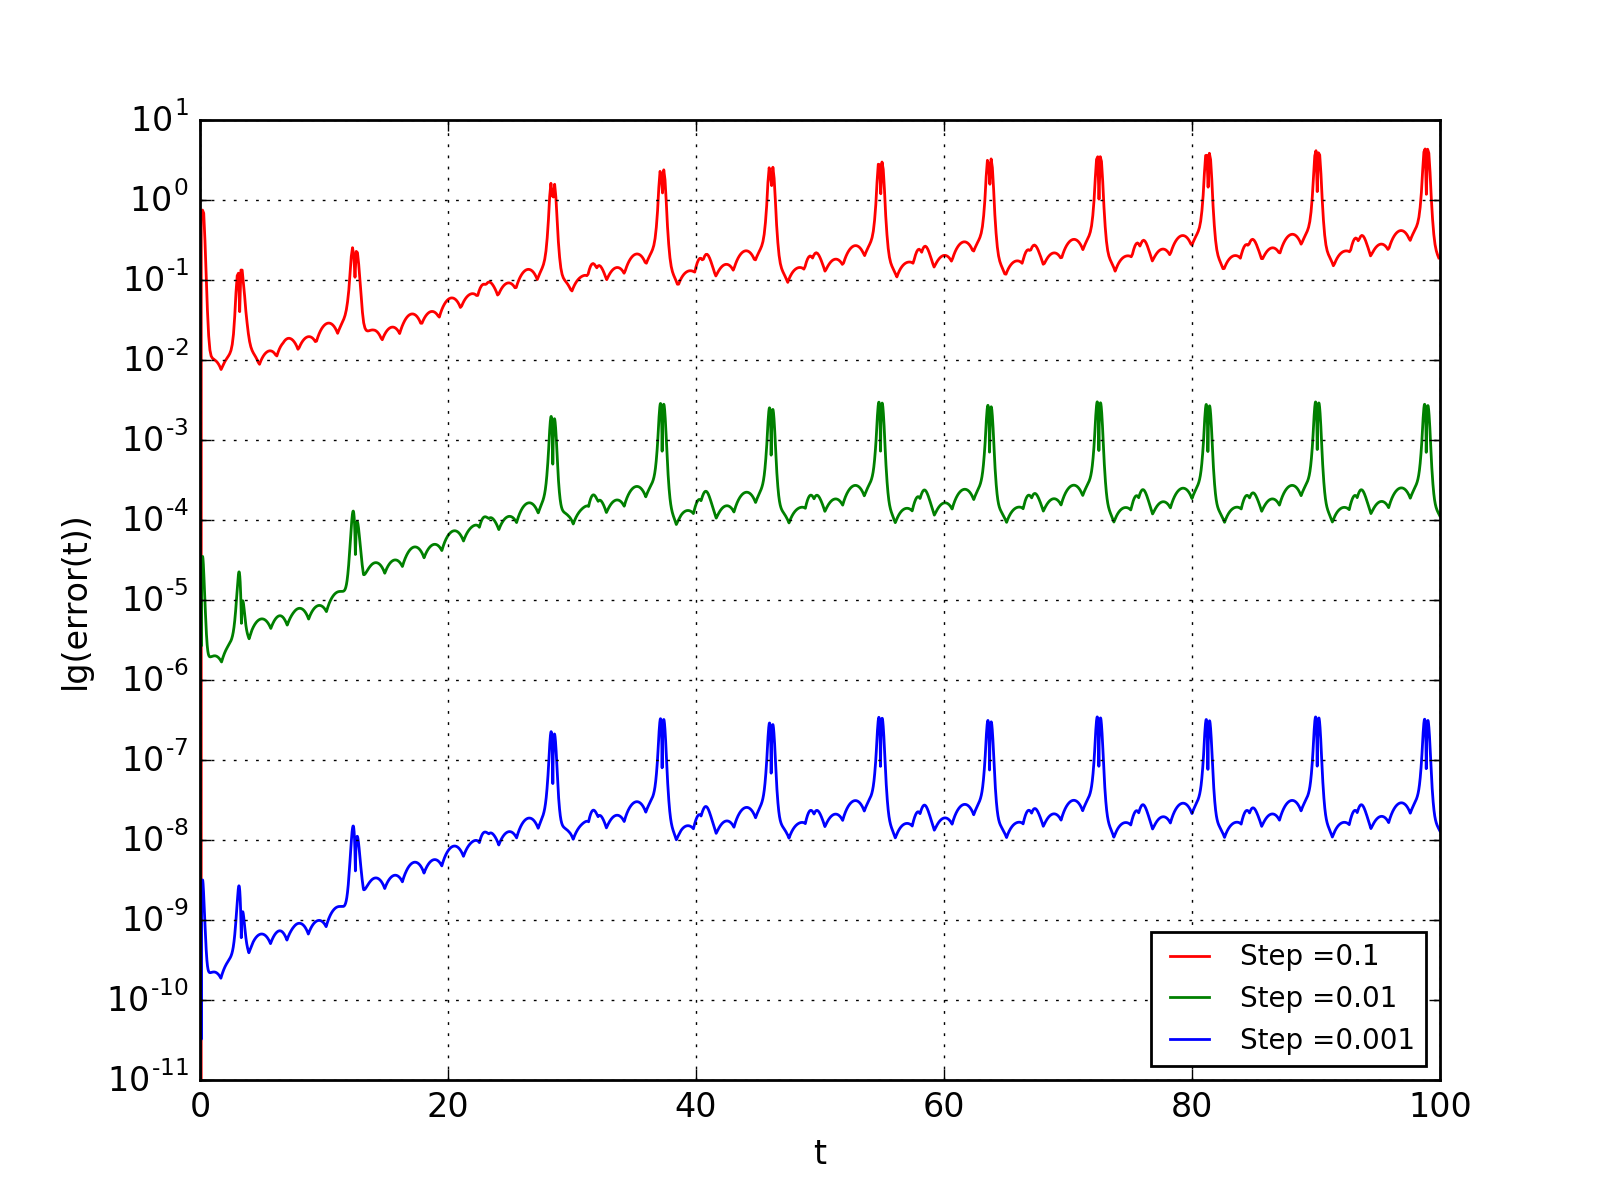
\includegraphics[width=0.75\textwidth]{../pictures/lab3_rossler_system.png}
	\caption{Ошибка интегрирования системы Рёсслера при различных значениях шага}
	\label{fig:rossler_system}
\end{figure}


\section{Исходный код}
\lstinputlisting[language=Python, numbers=left]{../scripts/lab3.py}

\end{document}
